\documentclass{article}

% if you need to pass options to natbib, use, e.g.:
% \PassOptionsToPackage{numbers, compress}{natbib}
% before loading nips_2017
%
% to avoid loading the natbib package, add option nonatbib:
% \usepackage[nonatbib]{nips_2017}
% \usepackage{nips_2018}


% if you need to pass options to natbib, use, e.g.:
% \PassOptionsToPackage{numbers, compress}{natbib}
% before loading nips_2017
%
% to avoid loading the natbib package, add option nonatbib:
% \usepackage[nonatbib]{nips_2017}

\usepackage{nips_2018}

% to compile a camera-ready version, add the [final] option, e.g.:
% \usepackage[final]{nips_2017}
%\usepackage{enumitem}
\usepackage[utf8]{inputenc} % allow utf-8 input
\usepackage[T1]{fontenc}    % use 8-bit T1 fonts
\usepackage{hyperref}       % hyperlinks
\usepackage{url}            % simple URL typesetting
\usepackage{booktabs}       % professional-quality tables
\usepackage{amsfonts}       % blackboard math symbols
\usepackage{nicefrac}       % compact symbols for 1/2, etc.
%\usepackage{microtype}      % microtypography
%\usepackage{svg}
% \usepackage{subfigure}
\usepackage{amsmath}
\usepackage{amssymb}
%\usepackage{comment}
\usepackage{graphicx}
%\usepackage{cancel}
\usepackage{amsthm}
\usepackage{natbib}
\usepackage{dsfont}
\usepackage{xcolor}
%\usepackage{ stmaryrd }

\usepackage{cleveref}
% \usepackage{dsfont}
% \usepackage{txfonts}
% \usepackage{stackengine}
\newcommand{\fint}{\int_{\Sp^{d-1}}}



\title{Sliced-Wasserstein Flows: Nonparametric Generative Modeling via Optimal Transport and MCMC\\ {\large SUPPLEMENTARY DOCUMENT}}

% The \author macro works with any number of authors. There are two
% commands used to separate the names and addresses of multiple
% authors: \And and \AND.
%
% Using \And between authors leaves it to LaTeX to determine where to
% break the lines. Using \AND forces a line break at that point. So,
% if LaTeX puts 3 of 4 authors names on the first line, and the last
% on the second line, try using \AND instead of \And before the third
% author name.

\author{
  David S.~Hippocampus\thanks{Use footnote for providing further
    information about author (webpage, alternative
    address)---\emph{not} for acknowledging funding agencies.} \\
  Department of Computer Science\\
  Cranberry-Lemon University\\
  Pittsburgh, PA 15213 \\
  \texttt{hippo@cs.cranberry-lemon.edu} \\
  %% examples of more authors
  %% \And
  %% Coauthor \\
  %% Affiliation \\
  %% Address \\
  %% \texttt{email} \\
  %% \AND
  %% Coauthor \\
  %% Affiliation \\
  %% Address \\
  %% \texttt{email} \\
  %% \And
  %% Coauthor \\
  %% Affiliation \\
  %% Address \\
  %% \texttt{email} \\
  %% \And
  %% Coauthor \\
  %% Affiliation \\
  %% Address \\
  %% \texttt{email} \\
}
\newcommand{\x}{\mathbf{x}}
\newcommand{\thb}{\mathbf{x}} 
\newcommand{\Ths}{{\cal X}} 
% \newcommand{\thb}{\boldsymbol{\theta}} 
% \newcommand{\Ths}{{\cal M}} 
\newcommand{\xe}{\tilde{\mathbf{x}}} 

\newcommand{\B}{\mathcal{B}}
\newcommand{\N}{\mathcal{N}}
\newcommand{\q}{\mathbf{q}}
\newcommand{\qc}{\mathbf{\bar{q}}}
\newcommand{\p}{\mathbf{p}}
\newcommand{\tb}{\mathbf{t}} 
\newcommand{\Ds}{{\cal D}} 

\newcommand{\M}{\mathbf{M}}
\newcommand{\stl}{l}
\newcommand{\Lo}{{\cal L}}
\newcommand{\Oc}{{\cal O}}
\newcommand{\Lot}{\tilde{\Lo}}
\newcommand{\y}{\mathbf{y}}
\newcommand{\Y}{{ Y}}
\newcommand{\D}{ {\cal D} }
\newcommand{\ba}[1]{b(#1,\alpha)}
\newcommand{\bta}[1]{\tilde{b}_{h,K}(#1,\alpha)}
\newcommand{\bha}[1]{\hat{b}(#1,\alpha)}
\newcommand{\rmd}{r}
\newcommand{\Sp}{\mathbb{S}}
\newcommand{\R}{\mathbb{R}}
\newcommand{\E}{\mathbb{E}}
\newcommand{\Pro}{\mathbb{P}}
\newcommand{\Pb}{\mathbf{P}}
\newcommand{\overbar}[1]{\mkern 1.5mu\overline{\mkern-1.5mu#1\mkern-1.5mu}\mkern 1.5mu}

\newcommand{\W}{{\cal W}_2}
\newcommand{\F}{{\cal F}}
\newcommand{\PS}{{\cal P}}
\newcommand{\He}{{\cal H}}
\newcommand{\SW}{{\cal S}{\cal W}_2}
\newcommand{\TV}{\textnormal{TV}}
\newcommand{\KL}{\textnormal{KL}}
\newcommand{\muh}{\hat{\mu}}

\newtheorem{thm}{Theorem}
\newtheorem{remark}{Remark}
\newtheorem{cor}{Corollary}
\newtheorem{lemma}{Lemma}
\newtheorem{prop}{Proposition}

\DeclareMathOperator*{\argmin}{arg\min}
\DeclareMathOperator*{\argmax}{arg\max}

\DeclareMathOperator{\cB}{\overline{B}}


\newcommand{\tmpeqno}{{\color{red} (TEMPEQ) }}

\newcommand{\umut}[1]{{\color{red} (#1)} }

\DeclareMathOperator{\sign}{sign}
\newcommand{\sas}{{\cal S} \alpha {\cal S} }

% \newcommand{\pb}{\bar{{\cal P}}}
% \newcommand{\pt}{\tilde{{\cal P}}}

\newcommand{\pb}{{\cal P}^\x}
\newcommand{\pt}{{\cal P}^\y}

% \newcommand{\ab}{\bar{{\cal A}}}
% \newcommand{\at}{\tilde{{\cal A}}}

\newcommand{\ab}{{\cal A}^\x}
\newcommand{\at}{{\cal A}^\y}

\usepackage{cleveref}


% \newtheoremstyle{exampstyle}
%   {\topsep} % Space above
%   {0} % Space below
%   {} % Body font
%   {} % Indent amount
%   {\bfseries} % Theorem head font
%   {.} % Punctuation after theorem head
%   {0pt} % Space after theorem head
%   {} % Theorem head spec (can be left empty, meaning `normal')

% \theoremstyle{exampstyle} 

\newtheorem{assumption}{\textbf{H}\hspace{-3pt}}
\Crefname{assumption}{\textbf{H}\hspace{-3pt}}{\textbf{H}\hspace{-3pt}}
\crefname{assumption}{\textbf{H}}{\textbf{H}}



\newcommand{\insertimage}[4]{ % scale, filename, caption, label
\begin{figure}[t]
\centering
\includegraphics[scale=#1, clip=true]{figures/#2}
\caption{#3}
\label{#4}
\end{figure}
}

\newcommand{\insertimageC}[5]{ % scale, filename, caption, label, location
\begin{figure}[#5]
\centering
\includegraphics[width=#1\linewidth, clip=true]{figures/#2}
%\vspace{-1.5em}
\caption{#3}
%\vspace{-0.5em}
\label{#4}
\end{figure}
}

%\setlength{\belowcaptionskip}{-10pt}
%\captionsetup[figure]{calcwidth = 0.95\linewidth,skip=10pt}
% \setlength{\abovecaptionskip}{-10pt}

\newcommand{\insertimageStar}[5]{ % scale, filename, caption, label, location
\begin{figure*}[#5]
\centering
\includegraphics[width=#1\linewidth, clip=true]{figures/#2}
\caption{#3}
%\vspace{-0.5em}
\label{#4}
\end{figure*}
}

\newcommand{\insertimageAsSubfig}[5]{ % scale, filename, caption, label,
\begin{figure}[#5]
\begin{center}
\subfigbottomskip =-4in
\subfigure{
\includegraphics[width=#1\columnwidth]{figures/#2}
\label{#4}
}
\end{center}
\subfigbottomskip =-4in
\caption{#3}
\label{#4}
\end{figure}
}


\newcommand{\floor}[1]{\left\lfloor #1 \right\rfloor}
\newcommand{\ceil}[1]{\left\lceil #1 \right\rceil}


\usepackage{xr}
\externaldocument{nips_2018_sketchmcmc}

\setcounter{equation}{0}
\setcounter{figure}{0}
\setcounter{table}{0}
\setcounter{page}{1}
% %\makeatletter
 \renewcommand{\theequation}{S\arabic{equation}}
 \renewcommand{\thefigure}{S\arabic{figure}}
 \renewcommand{\thelemma}{S\arabic{lemma}}
\renewcommand{\theassumption}{S\arabic{assumption}}
 \renewcommand{\thethm}{S\arabic{thm}}
 \renewcommand{\theprop}{S\arabic{prop}}

\usepackage[shortlabels]{enumitem}


\begin{document}
% \nipsfinalcopy is no longer used

\maketitle

% 
% %!TEX root = ./nips_2018_sketchmcmc_supp.tex

\section{Gradient flows info -- to be merged with the next section}

In order to prove that the path $(\rho_t)_t$ solves a PDE for a given gradient flow, one first needs to show that there exits a path $(\rho_t)_t$ that appears as the limit of the solution of a \emph{time-discretized} problem \cite{jordan1998variational,santambrogio2017euclidean}. In particular, we need to show that for $\mu_t(dx) = \rho_t(x)dx$, $(\mu_t)_{t\geq 0}$ is point-wise limit of a family $(\mu_t^h)_{t\geq 0}$, where $\mu_t^h = \mu_{kh}^h$ for $t \in [kh, (k+1)h)$ (i.e.\ piece-wise constant), and $\mu_{(k+1)h}^h$ solves the following optimization problem:
\begin{align}
\mu^{h}_{(k+1)h} = \argmin_\mu \mathcal{G}(h, k , \mu, \mu^h_{kh}),  %\triangleq \mathcal{F}(\mu) + \frac{1}{2h}\W(\mu, \mu^k) %\argmin_\rho \Bigl\{ \F(\rho) + \frac1{2h}\W^2(\rho, \rho_k^h) \Bigr\},
\end{align} 
where,
\begin{align}
\mathcal{G}(h, k , \mu_+, \mu_-) \triangleq \mathcal{F}(\mu_+) + \frac{1}{2h}\W(\mu_+, \mu_-).
\end{align}
If $(\mu_t)_{t\geq 0}$ appears as the limiting curve $\lim_{h\rightarrow 0}(\mu_t^h)_{t\geq 0}$, then $(\mu_t)_{t\geq 0}$ is called a \emph{generalized minimizing movement} \cite{santambrogio2017euclidean,bonnotte2013unidimensional}. Proving that $(\mu_t)_{t\geq 0}$ is a minimizing movement ensures that the gradient flow $\partial_t \mu_t = - \nabla_{\W} \F(\mu_t)$ exists; however, the form of the vector field $v$ in \eqref{eqn:pde} can only be determined by further analysis.
%!TEX root = ./aistats_2019_sketchmcmc_supp.tex

\section{Proof of Theorem~\ref{thm:continuity}}

We first need to generalize \cite[Lemma 5.4.3]{bonnotte2013unidimensional} to distribution $\rho \in \mrl^{\infty}(\cB(0,r))$, $r >0$.
\begin{thm} \label{thm:implicit_step}
 Let $\nu$ be a probability measure on $\cB(0,1)$ with a strictly positive smooth density. Fix a time step $h > 0$, regularization constant $\lambda > 0$ and a radius $r > \sqrt{d}$. For any probability measure $\mu_0$ on $\cB(0, r)$ with density $\rho_0 \in \mrl^{\infty}(\cB(0, r))$, there is a probability measure $\mu$ on $\cB(0,r)$ minimizing:
\[
\mathcal{G}(\mu) = \mcf^{\nu}_{\lambda} (\mu) + \frac{1}{2h} \W^2(\mu, \mu_0) ,
\]
where $\mcf^{\nu}_\lambda$ is given by \eqref{eqn:sw_optim}.
Moreover the optimal $\mu$ has a density $\rho$ on $\cB(0,r)$ and:
\begin{equation} \label{ineq:inf_norm_bound}
||\rho||_{\mrl^{\infty}} \leq (1 + h/\sqrt{d})^d ||\rho_0||_{\mrl^{\infty}}.
\end{equation}
\end{thm}
\begin{proof}
The set of measures supported on $\cB(0,r)$ is compact in the topology given by $\W$ metric. Furthermore by \cite[Lemma 9.4.3]{ambrosio2008gradient} $\He$ is lower semicontinuous on $(\PS(\cB(0,r)),\W)$. Since by \cite[Proposition 5.1.2, Proposition 5.1.3]{bonnotte2013unidimensional}, $\SW$ is a distance  on $\PS(\cB(0,r))$, dominated by $d^{-1/2} \W$, we have:
\[
|\SW(\pi_0, \nu) - \SW(\pi_1, \nu)| \leq \SW(\pi_0, \pi_1) \leq \frac{1}{\sqrt{d}}\W(\pi_0, \pi_1).
\]
The above means that $\SW(\cdot, \nu)$ is continuous with respect to topology given by $\W$, which implies that $\SW^2(\cdot, \nu)$ is continuous in this topology as well. Therefore $\mcg : \PS(\cB(0,r)) \to \ocint{-\infty,\plusinfty}$ is a lower semicontinuous function on the compact set $(\PS(\cB(0,r)),\W)$. Hence there exists a minimum  $\mu$ of $\mcg$ on $\mathcal{P}(\cB(0,r))$. Furthermore, since $\mch(\pi) = +\infty$  for measures $\pi$ that do not admit a density with respect to Lebesgue measure, the measure $\mu$ must admit a density $\rho$.

If $\rho_0$ is smooth and positive on $\cB(0,r)$, the inequality \ref{ineq:inf_norm_bound} is true by \cite[Lemma 5.4.3.]{bonnotte2013unidimensional} When $\rho_0$ is just in $\mrl^{\infty}(\cB(0,r))$, we proceed by smoothing. 
For $t \in (0,1]$, let $\rho_t$ be a function obtained by convolution of $\rho_0$ with a Gaussian kernel $(t,x,y) \mapsto (2\pi)^{d/2} \exp(\norm[2]{x-y}/2)$, restricting the result to $\cB(0,r)$ and normalizing to obtain a probability density. Then $(\rho_t)_{t}$ are smooth positive densities, and it is easy to see that $\lim_{t \rightarrow 0} ||\rho_t||_{\mrl^{\infty}} \leq ||\rho_0||_{\mrl^{\infty}}$. Furthermore, if we denote by $\mu_t$ the measure on $\cB(0,r)$ with density $\rho_t$, then $\mu_t$ converge weakly to $\mu_0$.
%Let $\mu_t$ be the heat flow on $\cB(0,r)$ starting from $\mu_0$ ([[some ref on existance?]]). 
%Then for any $t > 0$, $\mu_t$ has a smooth density $\rho_t$ such that  
For $t \in (0, 1]$ let $\hat{\mu}_t$ be the minimum of $ \mcf^{\nu}_{\lambda}(\cdot) + \frac{1}{2h} \W^2(\cdot, \mu_t)$, and let $\hat{\rho}_t$ be the density of $\hat{\mu}_t$. Using \cite[Lemma 5.4.3.]{bonnotte2013unidimensional} we get 
\[
||\hat{\rho}_t ||_{\mrl^{\infty}} \leq (1 + h\sqrt{d})^d ||\rho_t||_{\mrl^{\infty}}.
\]
so $\hat{\rho_{t}}$ lies in a ball of finite radius in $\mrl^{\infty}$.  Using compactness of $\mathcal{P}(\cB(0,r))$ in weak topology and compactness of closed ball in $\mrl^{\infty}(\cB(0,r))$ in weak star topology, we can choose a subsequence $\hat{\mu}_{t_k} , \hat{\rho}_{t_k}$, $\lim_{k \to \plusinfty} t_k =0$, that converges along that subsequence to limits $\hat{\mu}$, $\hat{\rho}$. Obviously $\hat{\rho}$ is the density of $\hat{\mu}$, since for any continuous function $f$  on $\cB(0,r)$ we have:
\[
\int \hat{\rho} f dx = \lim_{k \rightarrow \infty} \int \rho_{t_k} f dx = \lim_{k \rightarrow \infty} \int f d\mu_{t_k} = \int f d\mu.
\]
Furthermore, since $\hat{\rho}$ is the weak star limit of a bounded subsequence, we have:
\[
||\hat{\rho} ||_{\mrl^{\infty}} \leq \limsup_{k \rightarrow \infty}(1 + h\sqrt{d})^d ||\rho_{t_k}||_{\mrl^{\infty}} \leq (1 + h\sqrt{d})^d ||\rho_0||_{\mrl^{\infty}}.
\]
To finish, we just need to prove that $\hat{\mu}$ is a minimum of $\mcg$. We remind our reader, that we already established existence of some minimum $\mu$ (that might be different from $\hat{\mu}$). Since $\hat{\mu}_{t_k}$ converges weakly to $\hat{\mu}$ in $\mathcal{P}(\cB(0,r))$, it implies convergence  in $\W$ as well since $\cB(0,r)$ is compact. Similarly $\mu_{t_k}$ converges to $\mu_0$ in $\W$. Using the lower semicontinuity of $\mcg$ we now have:
\[
\begin{aligned}
\mcf^{\nu}_{\lambda}(\hat{\mu}) + \frac{1}{2h} \W^2(\hat{\mu}, \mu_0)  & \leq \liminf_{k \rightarrow \infty} \left( \mcf^{\nu}_{\lambda}(\hat{\mu}_{t_k}) + \frac{1}{2h} \W^2(\hat{\mu}_{t_k} , \mu_0) \right) \\
& \leq \liminf_{k \rightarrow \infty}  \mcf^{\nu}_{\lambda}(\mu) + \frac{1}{2h} \W^2(\mu , \mu_{t_k})   \\
& + \frac{1}{2h}  \W^2(\hat{\mu}_{t_k}, \mu_0) - \frac{1}{2h} \W^2(\hat{\mu}_{t_k}, \mu_{t_k})   \\
& = \mcf^{\nu}_{\lambda} (\mu) + \frac{1}{2h} \W^2(\mu, \mu_0) ,
\end{aligned}
\]
where the second inequality comes from the fact, that $\hat{\mu}_{t_k}$ minimizes $\mcf^{\nu}_{\lambda}(\cdot) + \frac{1}{2h}\W^2(\cdot, \mu_{t_k})$. From the above inequality and previously established facts, it follows that $\hat{\mu}$ is a minimum of $\mcg$ with density satisfying \ref{ineq:inf_norm_bound}.
\end{proof}

\begin{definition} \textbf{Minimizing movement scheme}
  \label{def:mini_move}
Let $r >0$ and  $\mcf : \mathbb{R_+} \times \PS(\cB(0,r)) \times \PS(\cB(0,r))\rightarrow \rset$ be a functional. Let $\mu_0 \in \PS(\cB(0,r))$ be a starting point. For $h> 0$ a piecewise constant trajectory $\mu^h : [0, \infty) \rightarrow \PS(\cB(0,r))$ for $\mcf$ starting at $\mu_0$ is a function such that:
\begin{itemize}
\item $\mu^h(0) = \mu_0$.
\item $\mu^h$ is constant on each interval $[nh, (n+1)h)$, so $\mu^h(t) = \mu^h(nh)$ with $n = \lfloor t/h \rfloor$.
\item $\mu^h((n+1)h )$ minimizes the  functional $ \zeta  \mapsto \mcf(h,  \zeta ,\mu^h(nh))$, for all $n \in \nset$.
\end{itemize}
We say $\hat{\mu}$ is a minimizing movement scheme for $\mcf$ starting at $\mu_0$, if there exists a family of piecewise constant trajectory $(\mu^h)_{h >0}$ for $\mcf$ such that $\hat{\mu}$ is a pointwise limit of $\mu^h$ as $h$ goes to $0$, \ie~for all $t \in \rset_+$, $\lim_{h \to 0} \mu^h(t) = \mu(t)$ in $\PS(\cB(0,r))$. We say that $\tilde{\mu}$ is a generalized minimizing movement for  $\mcf$ starting at $\mu_0$, if there exists a family of piecewise constant trajectory $(\mu^h)_{h >0}$ for $\mcf$ and  a sequence $(h_n)_n$, $\lim_{n \to \infty} h_n = 0$, such that $\mu^{h_n}$ converges pointwise to $\tilde{\mu}$.
\end{definition}


\begin{thm} \label{thm:existance_gmm_scheme}
Let $\nu$ be a probability measure on $\cB(0,1)$ with a strictly positive smooth density. Fix a regularization constant $\lambda > 0$ and radius $r > \sqrt{d}$. Given an absolutely continuous measure $\mu_0 \in \mathcal{P}(\cB(0,r))$ with density $\rho_0 \in \mrl^{\infty}(\cB(0,r))$, there is a generalized minimizing movement scheme $(\mu_t)_t$ in $\mathcal{P}(\cB(0,r))$ starting from $\mu_0$ for the functional defined by 
\begin{equation} \label{gmm:sw_ent_functional}
\mcf^{\nu}(h, \mu_+, \mu_-) = \mcf^{\nu}_{\lambda}(\mu_+) + \frac{1}{2h}\W^2(\mu_+, \mu_-).
\end{equation}
Moreover for any time $t > 0$, the probability measure $\mu_t = \mu(t)$ has density $\rho_t$ with respect to the Lebesgue measure and:
\begin{equation}
  \label{eq:bound:existance_gmm_scheme}
||\rho_t||_{\mrl^{\infty}} \leq e^{d t\sqrt{d}} ||\rho_0||_{\mrl^{\infty}} .  
\end{equation}
\end{thm}
\begin{proof}
We start by noting, that by \ref{thm:implicit_step} for any $h > 0$ there exists a piecewise constant trajectory $\mu^h$ for \ref{gmm:sw_ent_functional} starting at $\mu_0$. Furthermore for $t \geq 0$ measure $\mu_t^h = \mu^h(t)$ has density $\rho_t^h$, and:
\begin{equation} \label{ineq:dens_bound}
||\rho_t^h||_{\mrl^{\infty}} \leq e^{d \sqrt{d} (t+ h)} ||\rho_0||_{\mrl^{\infty}}.
\end{equation}
Let us choose $T > 0$. We denote $\rho^h(t,x) = \rho_t^h(x)$. 
%Also, for $h > 0$ we define a measure $\rho^h$ on $[0, T] \times \cB(0,r)$ by:
%\[
%\int \xi(t,x) d\rho^h(t,x) dx dt = \frac{1}{T} \int_0^T \int \xi(t,x) d\rho_t^h(x dx) dt 
%\]
%for all continuous and bounded functions $\xi$. 
For $ h \leq 1$, the functions $\rho^h$ lie in a ball in $\mrl^{\infty}([0,T] \times \cB(0,r))$, so from Banach-Alaoglu theorem there is a sequence $h_n$ converging to $0$, such that $\rho^{h_n}$ converges in weak-star topology in $\mrl^{\infty}([0,T] \times \cB(0,r))$ to a certain limit $\rho$. Since $\rho$ has to be nonnegative except for a set of measure zero, we assume $\rho$ is nonnegative. We denote $\rho_t(x) = \rho(t,x)$. We will prove that for almost all $t$, $\rho_t$ is a probability density and $\mu_{t}^{h_n}$ converges in $\W$ to a measure $\mu_t$ with density $\rho_t$.

First of all, for almost all $t \in [0,T]$, $\rho_t$ is a probability density, since for any Borel set $A \subseteq [0,T]$ the indicator of set $A \times \cB(0,r)$ is integrable, and hence by definition of the weak-star topology:
\[
\int_A \int_{\cB(0,r)} \rho_t(x) dx dt = \lim_{n \rightarrow \infty} \int_A \int_{\cB(0,r)} \rho_t^{h_n}(x) dx dt,
\]
and so we have to have $\int \rho_t(x) dx = 1$ for almost all $t \in [0,T]$. Nonnegativity of $\rho_t$ follows from nonnegativity of $\rho$. 

We will now prove, that for almost all $t \in [0,T]$ the measures $\mu_t^{h_n}$ converge to a measure with density $\rho_t$. Let $t \in (0,T)$, take $\delta < \min(T-t, t)$ and $\zeta \in \rmc^1(\cB(0,r))$. We have:
\begin{multline} \label{ineq:mu_t_conv_bound}
\left| \int_{\cB(0,r)} \zeta d\mu_t^{h_n} - \int_{\cB(0,r)} \zeta d\mu_t^{h_m} \right| \leq \\ \left| \int_{\cB(0,r)} \zeta d\mu_t^{h_n} - \frac{1}{2\delta} \int_{t - \delta}^{t + \delta} \int_{\cB(0,r)} \zeta d\mu_s^{h_n} ds \right| + 
\left| \int_{\cB(0,r)} \zeta d\mu_t^{h_m} - \frac{1}{2\delta} \int_{t - \delta}^{t + \delta} \int_{\cB(0,r)} \zeta d\mu_s^{h_m} ds \right| +  \\
\left| \frac{1}{2\delta} \int_{t - \delta}^{t + \delta} \int_{\cB(0,r)} \zeta d\mu_s^{h_m} ds - \frac{1}{2\delta} \int_{t - \delta}^{t + \delta} \int_{\cB(0,r)} \zeta d\mu_s^{h_n} ds \right|.
\end{multline}

Because $\mu_t^{h_n}$ have densities $\rho_t^{h_n}$ and both $\rho^{h_n}$, $\rho^{h_m}$ converge to $\rho$ in weak-star topology, the last element of the sum on the right hand side converges to zero, as $n,m \rightarrow \infty$. Next, we get a bound on the other two terms.


First, if we denote by $\gamma$ the optimal transport plan between $\mu_t^{h_n}$ and $\mu_s^{h_n}$, we have:
\begin{multline} \label{ineq:expectation_W2_bound}
\left| \int_{\cB(0,r)} \zeta d\mu_t^{h_n} - \int_{\cB(0,r)} \zeta d\mu_s^{h_n} \right|^2 \leq \int_{\cB(0,r) \times \cB(0,r)} \left| \zeta(x) - \zeta(y) \right|^2 d\gamma(x,y) \leq ||\nabla \zeta||_{\infty}^2 \W^2(\mu_t^{h_n}, \mu_s^{h_n}).
\end{multline}
In addition, for $n_t = \lfloor t/h_n \rfloor$ and $n_s = \lfloor s/h_n \rfloor$ we have $\mu_t^{h_n} = \mu_{n_t h_n}^{h_n}$ and $\mu_s^{h_n} = \mu_{n_s h_n}^{h_n}$. For all $k \geq 0$ we have:
\begin{equation}
  \label{eq:wasser_bound_1}
\W^2(\mu_{kh_n}^{h_n}, \mu_{(k+1)h_n}^{h_n}) \leq 2h_n(\mcf^{\nu}_{\lambda}(\mu_{kh_n}^{h_n}) - \mcf^{\nu}_{\lambda}(\mu_{(k+1)h_n}^{h_n})  .  
\end{equation}
Using this result and \eqref{ineq:expectation_W2_bound} and assuming without loss of generality $n_t \leq n_s$, from the Cauchy-Schwartz inequality we get:
\begin{align}
\nonumber
  \W^2(\mu_{t}^{h_n}, \mu_s^{h_n}) & \leq \left( \sum_{k= n_t}^{n_s-1} \W(\mu_{kh_n}^{h_n}, \mu_{(k+1)h_n}^{h_n}) \right)^2 \\
  \nonumber
                                   & \leq |n_t - n_s|\sum_{k=n_t}^{n_s 1} \W^2(\mu_{kh_n}^{h_n}, \mu_{(k+1)h_n}^{h_n}) \\
    \label{eq:wasser_bound_2}
& \leq 2h_n|n_t - n_s|(\mcf^{\nu}_{\lambda}(\mu_{n_t h_n}^{h_n}) - \mcf^{\nu}_{\lambda}(\mu_{n_s h_n}^{h_n}))  \leq 2C(|t-s| + h_n),
\end{align}
where we used for the last inequality, denoting $C = \mcf^{\nu}_{\lambda}(\mu_0) - \min_{\PS(\cB(0,r))} \mcf^{\nu}_{\lambda}$, that $(\mcf^{\nu}_{\lambda}(\mu_{kh_n}^{h_n}))_n$ is non-increasing by \eqref{eq:wasser_bound_1} and $\min_{\PS(\cB(0,r))} \mcf^{\nu}_{\lambda}$ is finite since $ \mcf^{\nu}_{\lambda}$ is lower semi-continuous.
Finally, using Jensen's inequality, the above bound and \ref{ineq:expectation_W2_bound} we get:
\[
\begin{aligned}
\left| \int_{\cB(0,r)} \zeta d\mu_t^{h_n} - \frac{1}{2\delta} \int_{t - \delta}^{t + \delta} \int_{\cB(0,r)} \zeta d\mu_s^{h_n} ds \right|^2 & \leq \frac{1}{2\delta} \int_{t - \delta}^{t + \delta} \left| \int_{\cB(0,r)} \zeta d\mu_{t}^{h_n} - \int_{\cB(0,r)} \zeta d\mu_s^{h_n} \right|^2 ds \\
& \leq \frac{C ||\nabla \zeta||_{\infty}^2}{\delta} \int_{t-\delta}^{t+\delta} (|t-s| +h_n) ds \\
& \leq 2C ||\nabla \zeta||_{\infty}^2 (h_n + \delta).
\end{aligned}
\]
Together with \eqref{ineq:mu_t_conv_bound}, when taking $\delta = h_n$, this result means that $\int_{\cB(0,r)} \zeta d\mu_t^{h_n}$ is a Cauchy sequence for all $t \in (0, T)$. On the other hand, since $\rho^{h_n}$ converges to $\rho$ in weak-star topology on $\mrl^{\infty}$, the limit of $\int_{\cB(0,r)} \zeta d\mu_t^{h_n}$ has to be $\int_{\cB(0,r)} \zeta(x) \rho_t(x) dx$ for almost all $t \in (0,T)$. This means that for almost all $t \in [0,T]$ sequence $\mu_{t}^{h_n}$ converges to a measure $\mu_t$ with density $\rho_t$.

Let $ S \in [0,T]$ be the set of times such that for $t \in S$ sequence $\mu_{t}^{h_n}$ converges to $\mu_t$. As we established almost all points from $[0,T]$ belong to $S$. Let $ t \in [0,T] \setminus S$. Then, there exists a sequence of times $t_k \in S$ converging to $t$, such that $\mu_{t_k}$ converge to some limit $\mu_t$. We have:
\[
\W(\mu_t^{h_n}, \mu_t) \leq \W(\mu_{t}^{h_n}, \mu_{t_k}^{h_n}) + \W(\mu_{t_k}^{h_n}, \mu_{t_k}) + \W(\mu_{t_k}, \mu_t).
\]
From which we have for all $k \geq 1$:
\[
\limsup_{n \rightarrow \infty} \W(\mu_{t}^{h_n}, \mu_t) \leq \W(\mu_{t_k}, \mu_t) + \limsup_{n\rightarrow \infty} \W(\mu_t^{h_n}, \mu_{t_k}^{h_n}),
\]
and using \eqref{eq:wasser_bound_2}, we get $\mu_{t}^{h_n} \rightarrow \mu_t$. Furthermore, the measure $\mu_t$ has to have density, since $\rho_{t}^{h_n}$ lie in a ball in $\mrl^{\infty}(\cB(0,r))$, so we can choose a subsequence of $\rho_t^{h_n}$ converging in weak-star topology to a certain limit $\hat{\rho}_t$, which is the density of $\mu_t$. 

We use now the diagonal argument to get convergence for all $t >0$. Let $(T_k)_{k=1}^{\infty}$ be a sequence of times increasing to infinity. Let $h_{n}^1$ be a sequence converging to $0$, such that $\mu_t^{h_n^1}$ converge to $\mu_t$ for all $t \in [0, T_1]$. Using the same arguments as above, we can choose a subsequence $h_n^2$ of $h_n^1$, such that $\mu_{t}^{h_n^2}$ converges to a limit $\mu_t$ for all $t \in [0, T_2]$. Inductively, we construct subsequences $h_{n}^k$, and in the end take $h_n = h_n^n$. For this subsequence we have that $\mu_t^{h_n}$ converges to $\mu_t$ for all $t > 0$, and $\mu_t$ has a density satisfying the bound from the statement of the theorem.

Finally, note that \eqref{thm:existance_gmm_scheme} follows from \eqref{ineq:dens_bound}.
\end{proof}

\begin{thm}
Let $(\mu_t)_{t \geq 0}$ be a generalized minimizing movement scheme given by Theorem~\ref{thm:existance_gmm_scheme} with initial distribution $\mu_0$ with density $\rho_0 \in \mrl(\cB(0,r))$. We denote by $\rho_t$ the density of $\mu_t$ for all $t \geq 0$. Then $\rho_t$ satisfies the continuity equation:
\[
\frac{\partial \rho_t}{\partial t} + \divop(v_t \rho_t) + \lambda \Delta \rho_t = 0 \,, \quad \quad \quad v_t(x) = - \int_{\mathbb{S}^{d-1}} \psi_{t, \theta}'(\langle x , \theta \rangle ) \theta d\theta ,
\]
in a weak sense, that is for all $\xi \in \rmc_c^{\infty} ([0, \infty)\times \cB(0,r))$ we have:
\[
\int_0^{\infty} \int_{\cB(0,r)} \left[\frac{\partial \xi}{\partial t}(t,x) - v_t \nabla \xi(t,x)  - \lambda \Delta \xi(t,x)\right] \rho_t(x) dx dt = -\int_{\cB(0,r)} \xi(0,x)\rho_0(x) dx.
\]
\end{thm}
\begin{proof}
Our proof is based on the proof of \cite[Theorem 5.6.1]{bonnotte2013unidimensional}. We proceed in five steps.

\begin{enumerate}[wide, labelwidth=!, labelindent=0pt,label=(\arabic*)]
\item Let $h_n \rightarrow 0$ be a sequence given by Theorem~\ref{thm:existance_gmm_scheme}, such that $\mu_t^{h_n}$ converges to $\mu_t$ pointwise. Furthermore we know that $\mu^{h_n}$ have densities $\rho^{h_n}$ that converge to $\rho$ in $\mrl^r$, for $r \geq 1$, and in weak-star topology in $\mrl^{\infty}$. Let $\xi \in \rmc_c^{\infty} ([0, \infty) \times \cB(0,r))$. We denote $\xi_{k}^n(x)  = \xi(kh_n, x)$. Using part $1$ of the proof of  \cite[Theorem 5.6.1]{bonnotte2013unidimensional}, we obtain:
\begin{multline} \label{thm:cont_proof_part1}
\int_{\cB(0,r)} \xi(0, x) \rho_0(x) dx + \int_0^{\infty} \int_{\cB(0,r)} \frac{\partial \xi}{\partial t}(t,x) \rho_t(x) dx dt \\
= \lim_{n \rightarrow \infty} - h_n \sum_{k=1}^{\infty} \int_{\cB(0,r)} \xi_k^n(x) \frac{\rho_{kh_n}^{h_n}(x) - \rho_{(k-1)h_n}^{h_n}(x) }{h_n} dx.
\end{multline}
\item Again, this part is the same as part $2$ of the proof of  \cite[Theorem 5.6.1]{bonnotte2013unidimensional}. For any $\theta \in \mathbb{S}^{d-1}$ we denote by $\psi_{t, \theta}$ the unique Kantorovich potential from $\theta_{\#}^{*}\mu_t$ to $\theta_{\#}^{*}\nu$, and by $\psi_{t, \theta}^{h_n}$ the unique Kantorovich potential from $\theta_{\#}^{*} \mu_t^{h_n}$ to $\theta_{\#}^{*} \nu$. Then, by the same reasoning as part $2$ of the proof of  \cite[Theorem 5.6.1]{bonnotte2013unidimensional}, we get:

\begin{multline} \label{thm:cont_proof_part2}
\int_0^{\infty} \int_{\cB(0,r)} \fint (\psi_{t, \theta})' (\langle \theta, x \rangle ) \langle \theta , \nabla \xi (x, t) \rangle d\theta d\mu_t(x) dt \\
= \lim_{n \rightarrow \infty} h_n \sum_{k=1}^{\infty} \int_{\cB(0,r)} \fint \psi_{kh_n, \theta}^{h_n} (\theta^{*}) \langle \theta, \nabla \xi_{k}^n \rangle d \theta d\mu_{kh_n}^{h_n}.
\end{multline}
\item  Since $\xi$ is compactly supported and smooth, $\Delta \xi$ is Lipschitz, and so for any $ t \geq 0$ if we take $k = \lfloor t/h_n \rfloor$ we get $| \Delta \xi_k^n(x) - \Delta \xi(t,x) | \leq C h_n$ for some constant $C$. Let $T > 0$ be such that $\xi(t,x) = 0 $ for $t > T$. We have:
\[
\left| \sum_{k=1}^{\infty} h_n \int_{\cB(0,r)} \Delta \xi_k^n(x) \rho_{kh_n}^{h_n}(x) dx - \int_{0}^{\plusinfty} \int_{\cB(0,r)} \Delta \xi(t,x) \rho_{t}^{h_n}(x) dx dt \right| \leq CTh_n .
\]
On the other hand,  we know, that $\rho^{h_n}$ converges to $\rho$ in weak star topology on $\mrl^{\infty}([0,T] \times \cB(0,r))$, and $\Delta \xi$ is bounded, so:
\[
\lim_{n \to \plusinfty}\left| \int_{0}^{\plusinfty} \int_{\cB(0,r)} \Delta \xi(t,x) \rho_{t}^{h_n}(x) dx dt - \int_{0}^{\plusinfty} \int_{\cB(0,r)} \Delta \xi (t,x) \rho_t(x) dx dt \right|= 0.
\]
Combining those two results give:
\begin{equation} \label{thm:cont_proof_part3}
\lim_{n \rightarrow \infty} h_n \sum_{k=1}^{\infty} \int_{\cB(0,r)} \Delta \xi_k^n(x) \rho_{kh_n}^{h_n}(x) dx = \int_{0}^{\plusinfty} \int_{\cB(0,r)} \Delta \xi (t,x) \rho_t(x) dx dt.
\end{equation}

\item 
  Let $\phi_{k}^{h_n}$ denote the unique Kantorovich potential from $\mu_{kh_n}^{h_n}$ to $\mu_{(k-1)h_n}^{h_n}$. Using  \cite[Propositions 1.5.7 and 5.1.7]{bonnotte2013unidimensional}, as well as \cite[Equation (38)]{jordan1998variational} with $\Psi = 0$, and optimality of $\mu_{kh_n}^{h_n}$, we get:
\begin{multline} \label{thm:cont_proof_eq0}
\frac{1}{h_n} \int_{\cB(0,r)} \langle \nabla \phi_k^{h_n}(x) , \nabla \xi_{k}^n(x) \rangle d\mu_{kh_n}^{h_n}(x)   - \int_{\cB(0,r)} \fint (\psi_{kh_n}^{h_n})'(\theta^{*}) \langle \theta, \nabla \xi_k^n(x) \rangle d\theta d\mu_{kh_n}^{h_n}(x)\\ - \lambda \int_{\cB(0,r)}   \Delta \xi_k^n(x) d\mu_{kh_n}^{h_n}(x) ,
\end{multline}
which is the derivative of $\mcf^{\nu}_{\lambda}(\cdot) + \frac{1}{2h_n}\W^2(\cdot, \mu_{(k-1)h_n})$ in the direction given by vector field $\nabla \xi_k^n$ is zero.

Let $\gamma$ be the optimal transport between $\mu_{kh_n}^{h_n}$ and $\mu_{(k-1)h_n}^{h_n}$. Then:
\begin{equation} \label{thm:cont_proof_eq1}
\int_{\cB(0,r)} \xi_k^n(x) \frac{\rho_{kh_n}^{h_n}(x) - \rho_{(k-1)h_n}^{h_n}(x)}{h_n} dx = \frac{1}{h_n} \int_{\cB(0,r)} (\xi_k^n(y) - \xi_k^n(x)) d\gamma(x,y).
\end{equation}
\begin{equation} \label{thm:cont_proof_eq2}
\frac{1}{h_n}\int_{\cB(0,r)} \langle \nabla \phi_k^{h_n}(x) , \nabla \xi_k^n(x) \rangle d\mu_{kh_n}^{h_n}(x)  = \frac{1}{h_n} \int_{\cB(0,r)} \langle \nabla \xi_k^n(x), y-x \rangle d\gamma(x,y). 
\end{equation}
Since $\xi$ is $\rmc_c^{\infty}$, it has Lipschitz gradient. Let $C$ be twice the Lipschitz constant of $\nabla \xi$. Then we have $| \xi(y) - \xi(x) - \langle \nabla \xi(x), y-x \rangle | \leq C|x- y|^2$, and hence:
\begin{equation} \label{thm:cont_proof_eq3}
\int_{\cB(0,r)} |\xi_k^n(y) - \xi_k^n(x) - \langle \nabla \xi_k^n(x), y-x \rangle | d \gamma(x,y) \leq C\W^2( \mu_{(k-1)h_n}^{h_n}, \mu_{kh_n}^{h_n}).
\end{equation}
Combining \eqref{thm:cont_proof_eq1}, \eqref{thm:cont_proof_eq2} and \eqref{thm:cont_proof_eq3}, we get:
\begin{multline} \label{thm:cont_proof_eq4}
\left|\sum_{k=1}^{\infty} h_n \int_{\cB(0,r)} \xi_k^n(x) \frac{\rho_{kh_n}^{h_n} - \rho_{(k-1)h_n}^{h_n}}{h_n} dx  + 
\sum_{k=1}^{\infty} h_n\int_{\cB(0,r)} \langle \nabla \phi_k^{h_n} , \nabla \xi_k^n \rangle d\mu_{kh_n}^{h_n} \right| \\
\leq C\sum_{k=1}^{\infty} \W^2(\mu_{(k-1)h_n}^{h_n}, \mu_{kh_n}^{h_n}).
\end{multline}

As  some $\mcf^{\nu}_{\lambda}$ have a finite minimum on $\mathcal{P}(\cB(0,r))$, we have:
\begin{equation} \label{thm:cont_proof_eq5}
\begin{aligned}
\sum_{k=1}^{\infty} \W^2(\mu_{(k-1)h_n}^{h_n}, \mu_{kh_n}^{h_n}) & \leq  2 h_n \sum_{k=1}^{\infty} \mcf^{\nu}_{\lambda}(\mu_{(k-1)h_n}^{h_n}) - \mcf^{\nu}_{\lambda}(\mu_{kh_n}^{h_n}) \\ & \leq 2h_n \left(\mcf^{\nu}_{\lambda}(\mu_0) - \min_{\mathcal{P}(\cB(0,r))}\mcf^{\nu}_{\lambda} \right).
\end{aligned}
\end{equation}
and so the sum on the right hand side of the equation goes to zero as $n$ goes to infinity.

From \eqref{thm:cont_proof_eq4}, \eqref{thm:cont_proof_eq5} and \eqref{thm:cont_proof_eq0} we conclude:
\begin{multline} \label{thm:cont_proof_part4}
\lim_{n \rightarrow \infty} - h_n \sum_{k=1}^{\infty} \xi_k^n(x)\frac{\rho_{kh_n}^{h_n} - \rho_{(k-1)h_n}^{h_n}}{h_n} dx = \\
\lim_{n \rightarrow \infty} \left( h_n \sum_{k=1}^{\infty} \int_{\cB(0,r)} \fint \psi_{kh_n, \theta}^{h_n} (\theta^{*}) \langle \theta, \nabla \xi_{k}^n \rangle d \theta d\mu_{kh_n}^{h_n} + h_n \sum_{k=1}^{\infty} \int_{\cB(0,r)} \Delta \xi_k^n(x) \rho_{kh_n}^{h_n}(x) dx  \right),
\end{multline}
where both limits exist, since the difference of left hand side and right hand side of the equation goes to zero, while the left hand side converges to a finite value by \eqref{thm:cont_proof_part1}.
\item  Combining \eqref{thm:cont_proof_part1}, \eqref{thm:cont_proof_part2}, \eqref{thm:cont_proof_part3} and \eqref{thm:cont_proof_part4} we get the result.   
\end{enumerate}
%
\end{proof}

%%% Local Variables:
%%% mode: latex
%%% TeX-master: "nips_2018_sketchmcmc_supp"
%%% End:

%!TEX root = ./nips_2018_sketchmcmc_supp.tex

% \section{The Gradient Flow and the SDE}

% Let $\rho_t$ be the density of a measure $\mu_t$ with respect to the Lebesgue measure, such that $\mu_t(dx) = \rho_t(x) dx$. In this section, we will be interested in the following gradient flow in $\W$:
% \begin{align}
% \partial_t \rho_t &= - \nabla_{\W} \F_\lambda(\rho_t) \\
% &=  \nabla \cdot (\rho_t \> v_t) + \lambda \Delta \rho_t, \label{eqn:gradflow_reg}
% \end{align}
% where 
% \begin{align}
% v_t(x) \triangleq \nabla \Psi_t(x) = \int_{\Sp^{d-1}} \psi'_{t,\theta}(\langle \theta, x \rangle) \theta \> d\theta \label{eqn:idt_v}
% \end{align}
% and
% \begin{align}
% \Psi_t(x) \triangleq \int_{\mathbb{S}^{d-1}} \psi_{t,\theta}(\langle \theta, x \rangle) \> d\theta.
% \end{align}
% Here, $\psi_{t,\theta}$ denotes the Kantorovich potential between $\theta^*_{\#}\mu_t$ and $\theta^*_{\#}\nu$ and $d\theta$ represents the uniform probability measure on $\Sp^{d-1}$, such that $\int_{\Sp^{d-1}} d \theta = 1$.

% We now consider the modified flow given in \eqref{eqn:gradflow_reg}. We can observe that, this equation is the Fokker-Planck equation associated with the following stochastic differential equation (SDE):
% \begin{align}
% d X_t = - v_t(X_t) dt + \sqrt{2 \lambda } d W_t, \label{eqn:sde}
% \end{align}
% where $W_t$ denotes the standard Brownian motion.

\section{Proof of Proposition~\ref{prop:dist_statmeas}}

%
\begin{proof}
By Corollary 1.2 of \cite{bogachev2016distances}, for any $\epsilon > 0$ we have 
\begin{align}
\| \mu_t - \mu_t^\epsilon \|_{\TV}^2 &\leq \int_0^\infty \int_{\R^d} \Bigl| \Bigl(\frac{\sqrt{\lambda}}{\sqrt{\epsilon}}- \frac{\sqrt{\epsilon}}{\sqrt{\lambda}} \Bigr) \sqrt{2\epsilon}  \Bigr|^2 \frac{\|\nabla \rho^\epsilon_s(x)\|^2}{\rho^\epsilon_s(x)}  dx ds \\
&\leq  C \Bigl| \Bigl(\frac{\sqrt{\lambda}}{\sqrt{\epsilon}}- \frac{\sqrt{\epsilon}}{\sqrt{\lambda}} \Bigr) \sqrt{2\epsilon}  \Bigr|^2 \label{eqn:prop_interm} \\
&= \frac{2C}{\lambda} (\lambda - \epsilon)^2,
\end{align}
where \eqref{eqn:prop_interm} is obtained by the assumption. The desired result is obtained by taking the taking the limit of both sides. 
\end{proof}
%

\section{Proof of Lemma~\ref{lem:euler}}
%
%
\begin{proof}
We use the proof technique presented in \cite{dalalyan2017theoretical,raginsky17a}. Starting from the discrete-time process $(\bar{X}_k)_{k\in \mathbb{N}_+}$, we first define a continuous-time process $(Y_t)_{t\geq 0}$ that linearly interpolates $(\bar{X}_k)_{k\in \mathbb{N}_+}$, given as follows: 
\begin{align}
d Y_t = \tilde{v}_t(Y) dt + \sqrt{2 \lambda} dW_t, \label{eqn:sde_linear}
\end{align}
where $\tilde{v}_t(Y) \triangleq - \sum_{k=0}^{\infty} \hat{v}_k (Y_{kh}) \mathds{1}_{[kh, (k+1)h)}(t)$ and $\mathds{1}$ denotes the indicator function. It is easy to verify that for all $k \in \mathbb{N}_+$, we have $Y_{kh} = \bar{X}_k$. 

Let us denote the distributions of $(X_t)_{t \in [0,T]}$ and $(Y_t)_{t \in [0,T]}$ as $\pi_{X}^T$ and $\pi_{Y}^T$ with $T = Kh$. Then we can use Girsanov's formula to express the Kullback-Leibler (KL) divergence between these two distributions, given as follows:
\begin{align}
\KL (\pi_{X}^T || \pi_{Y}^T) &= \frac1{4 \lambda} \int_0^{Kh} \E[ \|v_t(Y_t) + \tilde{v}_t(Y) \|^2 ]  \> dt \\
&= \frac1{4 \lambda} \sum_{k=0}^{K-1} \int_{kh}^{(k+1)h} \E[ \|v_t(Y_t) + \tilde{v}_t(Y) \|^2 ] \> dt \\
&= \frac1{4 \lambda} \sum_{k=0}^{K-1} \int_{kh}^{(k+1)h} \E[ \|v_t(Y_t) - \hat{v}_{kh}(Y_{kh}) \|^2 ] \> dt.
\end{align}
% where we use the notation $\hat{v}_{kh} \equiv \hat{v}_{k}$ in order to illustrate the time index more explicitly. 
By using $v_t(Y_t) - \hat{v}_{kh}(Y_{kh}) = ( v_t(Y_t) - v_{kh}(Y_{kh})) + ( v_{kh}(Y_{kh}) - \hat{v}_{kh}(Y_{kh}))$, we obtain
%
\begin{align}
\nonumber \KL (\pi_{X}^T || \pi_{Y}^T) \leq& \frac1{2 \lambda} \sum_{k=0}^{K-1} \int_{kh}^{(k+1)h} \E[ \|v_t(Y_t) - {v}_{kh}(Y_{kh}) \|^2 ] \> dt \\
&+  \frac1{2 \lambda} \sum_{k=0}^{K-1} \int_{kh}^{(k+1)h} \E[ \|v_{kh}(Y_{kh}) - \hat{v}_{kh}(Y_{kh}) \|^2 ] \> dt \\
\nonumber \leq& \frac{L^2}{\lambda} \sum_{k=0}^{K-1} \int_{kh}^{(k+1)h} \bigl(\E[ \|Y_t - Y_{kh} \|^2 ] + (t-kh)^2 \bigr)  \> dt \\
&+  \frac1{2 \lambda} \sum_{k=0}^{K-1} \int_{kh}^{(k+1)h} \E[ \|v_{kh}(Y_{kh}) - \hat{v}_{kh}(Y_{kh}) \|^2 ] \> dt . \label{eqn:lem1_proof_interm}
\end{align}
The last inequality is due to the Lipschitz condition \Cref{asmp:lipschitz}.

Now, let us focus on the term $\E[ \|Y_t - Y_{kh} \|^2]$. By using \eqref{eqn:sde_linear}, we obtain:
\begin{align}
Y_t - Y_{kh} = - (t-kh) \hat{v}_{kh}(Y_{kh}) + \sqrt{2 \lambda (t-kh)} Z,
\end{align}
where $Z$ denotes a standard normal random variable. By adding and subtracting the term $-(t-kh) v_{kh}(Y_{kh})$, we have:
\begin{align}
Y_t - Y_{kh} = -(t-kh)v_{kh}(Y_{kh}) + (t-kh)(v_{kh}(Y_{kh}) - \hat{v}_{kh}(Y_{kh})) + \sqrt{2 \lambda (t-kh)} Z.
\end{align}
Taking the square and then the expectation of both sides yields:
\begin{align}
\nonumber \E[ \|Y_t - Y_{kh} \|^2] \leq& 3(t-kh)^2 \E[ \|v_{kh}(Y_{kh})\|^2] + 3 (t-kh)^2 \E[\|v_{kh}(Y_{kh}) - \hat{v}_{kh}(Y_{kh})\|^2] \\
&+ 6\lambda (t-kh)d.
\end{align}
As a consequence of \Cref{asmp:lipschitz} and \Cref{asmp:init_fun}, we have $\| v_t(x)\| \leq L\|x\|+B$ for all $t \geq 0$, $x\in \R^d$. Combining this inequality with \Cref{asmp:stochgrad}, we obtain:
\begin{align}
\nonumber \E[ \|Y_t - Y_{kh} \|^2] \leq& 6(t-kh)^2 (L^2 \E[ \|Y_{kh}\|^2] + B^2) + 6(t-kh)^2 (L^2 \E[ \|Y_{kh}\|^2] + B^2) \\
&+ 6\lambda (t-kh)d\\
=& 12(t-kh)^2 (L^2 \E[ \|Y_{kh}\|^2] + B^2) + 6\lambda (t-kh)d.
\end{align}
By Lemma 3.2 of \cite{raginsky17a}, we have $\E[ \|Y_{kh}\|^2] \leq C_0 \triangleq C_e +2  (1 \vee \frac1{m})(b+2B^2 + d \lambda)$, where $C_e$ denotes the entropy of $\mu_0$. Using this result in the above equation yields:
\begin{align}
\E[ \|Y_t - Y_{kh} \|^2] \leq& 12(t-kh)^2 (L^2 C_0 + B^2) + 6\lambda (t-kh)d. \label{eqn:lem_bound1}
\end{align}

We now focus on the term $\E[ \|v_{kh}(Y_{kh}) - \hat{v}_{kh}(Y_{kh}) \|^2 ]$ in \eqref{eqn:lem1_proof_interm}. Similarly to the previous term, we can upper-bound this term as follows:
\begin{align}
\E[ \|v_{kh}(Y_{kh}) - \hat{v}_{kh}(Y_{kh}) \|^2 ] \leq& 2 \delta(L^2 \E[\|Y_{kh}\|^2] + B^2) \\
\leq& 2 \delta(L^2 C_0 + B^2). \label{eqn:lem_bound2}
\end{align}

By using \eqref{eqn:lem_bound1} and \eqref{eqn:lem_bound2} in \eqref{eqn:lem1_proof_interm}, we obtain:
\begin{align}
\nonumber \KL (\pi_{X}^T || \pi_{Y}^T) \leq& \frac{L^2}{\lambda} \sum_{k=0}^{K-1} \int_{kh}^{(k+1)h} \bigl(12(t-kh)^2 (L^2 C_0 + B^2) + 6\lambda (t-kh)d +(t-kh)^2 \bigr) dt\\
&+  \frac1{2 \lambda} \sum_{k=0}^{K-1} \int_{kh}^{(k+1)h} 2 \delta(L^2 C_0 + B^2) \> dt \\
=& \frac{L^2 K}{\lambda} \Bigl( \frac{C_1 h^3}{3} + \frac{6 \lambda d h^2}{2} \Bigr) + \frac{C_2 \delta K h}{2\lambda},
\end{align}
where $C_1 = 12(L^2 C_0 + B^2)+1$ and $C_2 = 2 (L^2 C_0 + B^2)$.

Finally, by using the data processing and Pinsker inequalities, we obtain:
\begin{align}
\| \muh_{Kh} - \mu_{T} \|_{\TV}^2 \leq \| \pi_{X}^T - \pi_{Y}^T \|_{\TV}^2 \leq& \frac1{4} \KL (\pi_{X}^T || \pi_{Y}^T) \\
=& \frac{L^2 K}{4\lambda} \Bigl( \frac{C_1 h^3}{3} + 3 \lambda d h^2 \Bigr) + \frac{C_2 \delta K h}{8\lambda}.
\end{align}
This concludes the proof.
%
\end{proof}


\section{Proof of Theorem~\ref{thm:euler}}
%
\begin{proof}
By triangle inequality, we have that
\begin{align}
\| \muh_{Kh} - \nu_\lambda \|_{\TV} \leq \| \muh_{Kh} - \mu_{T} \|_{\TV} + \| \mu_{T} - \nu_\lambda \|_{\TV}.
\end{align}
Then the desired result is a direct consequence of Lemma~\ref{lem:euler} and assumption \Cref{asmp:sde_expconv}.
\end{proof}

\section{Proof of Corollary~\ref{coro:precision}}
\begin{proof}
Considering the bound given in Lemma~\ref{lem:euler}, the choices of $T$ and $h$ imply that
\begin{align}
\frac{L^2 K}{4\lambda} \Bigl( \frac{C_1 h^3}{3} + \frac{6 \lambda d h^2}{2} \Bigr) \leq \frac{\varepsilon^2}{4}, \quad \text{and} \quad C_3 \exp(-C_4 Kh \lambda) \leq \frac{\varepsilon}{2}. \label{eqn:cor_Th}
\end{align}
By combining \eqref{eqn:cor_Th} with the inequality $\sqrt{a+b}\leq \sqrt{a} + \sqrt{b}$, we obtain the desired result. 
\end{proof}

% \section{Discussion on the assumptions}

% \umut{This section will be rewritten.}

% \subsection{Conditions for the unique solution to the flow}

% The following conditions ensure that there is a unique solution to the flow given in \eqref{eqn:gradflow_reg}:
% \begin{assumption}
% \label{asmp:flowunq_1}
% There exists $p>d+2$ such that for every open ball $B \subset \R^d$, one has
% \begin{align}
% \int_0^T \int_B \|v_t(x)\|^p dx\> dt < \infty.
% \end{align}
% \end{assumption}
% %
% \begin{assumption}
% \label{asmp:flowunq_2}
% The initial measure $\mu_0$ has finite entropy, such that
% \begin{align}
% \int_{\R^d} \rho_0(x) \log \rho_0(x) dx < \infty,
% \end{align}
% where $\mu_0(dx) = \rho_0(x)dx$ and $\rho_0 \in L^1(\R^d)$.
% \end{assumption}
% %
% \begin{assumption}
% \label{asmp:flowunq_3}
% There exist $\alpha, \gamma, \delta, c, k \in \R_+$ such that for all $(t,x) \in [0,T] \times \R^d$ 
% \begin{align}
% \langle v_t(x), x \rangle \leq \gamma - (ck + \delta) \| x\|^{2k},
% \end{align}
% and 
% \begin{align}
% \label{asmp:flowunq_4}
% \|v_t(x)\| \leq \alpha \exp(\frac{c}{2} \|x\|^{2k}), \qquad \text{and} \qquad \int_{\R^d} \exp(\frac{c}{2}\|x\|^{2k} ) \mu_0(dx) < \infty.
% \end{align}
% \end{assumption}

% The following theorem ensures the uniqueness.
% \begin{thm}[Theorem 3.3 \cite{bogachev2007uniqueness}]
% Assume that \Cref{asmp:flowunq_1,asmp:flowunq_2,asmp:flowunq_3,asmp:flowunq_4} hold. Then, there exists a unique family $\{\mu_t, t\in(0,T]\}$ of probability measures on $\R^d$ solving \eqref{eqn:gradflow_reg}.
% \end{thm}

% \subsection{The assumptions of Proposition~\ref{prop:dist_statmeas}}

% The assumptions of Proposition~\ref{prop:dist_statmeas} can be satisfied if we further assume certain regularity assumptions on $v_t$. For more information and a discussion about these assumptions, we refer the reader to Remark 1.4 in \cite{bogachev2016distances} and \cite{bogachev2006global,bogachev2008estimates}.



%%% Local Variables:
%%% mode: latex
%%% TeX-master: "nips_2018_sketchmcmc_supp"
%%% End:

%!TEX root = ./aistats_2019_sketchmcmc_supp.tex


% \section{Visual Comparison with Existing Approaches}

% In this section, we provide the results presented in \cite{deshpande2018generative} for visual comparison. These results are obtained by running different IGM approaches on the MNIST dataset, namely GAN \cite{goodfellow2014generative}, Wasserstein GAN (W-GAN) \cite{arjovsky2017wasserstein} and the Sliced-Wasserstein Generator (SWG) \cite{deshpande2018generative}.

% \begin{figure}[h!]
% \centering
% 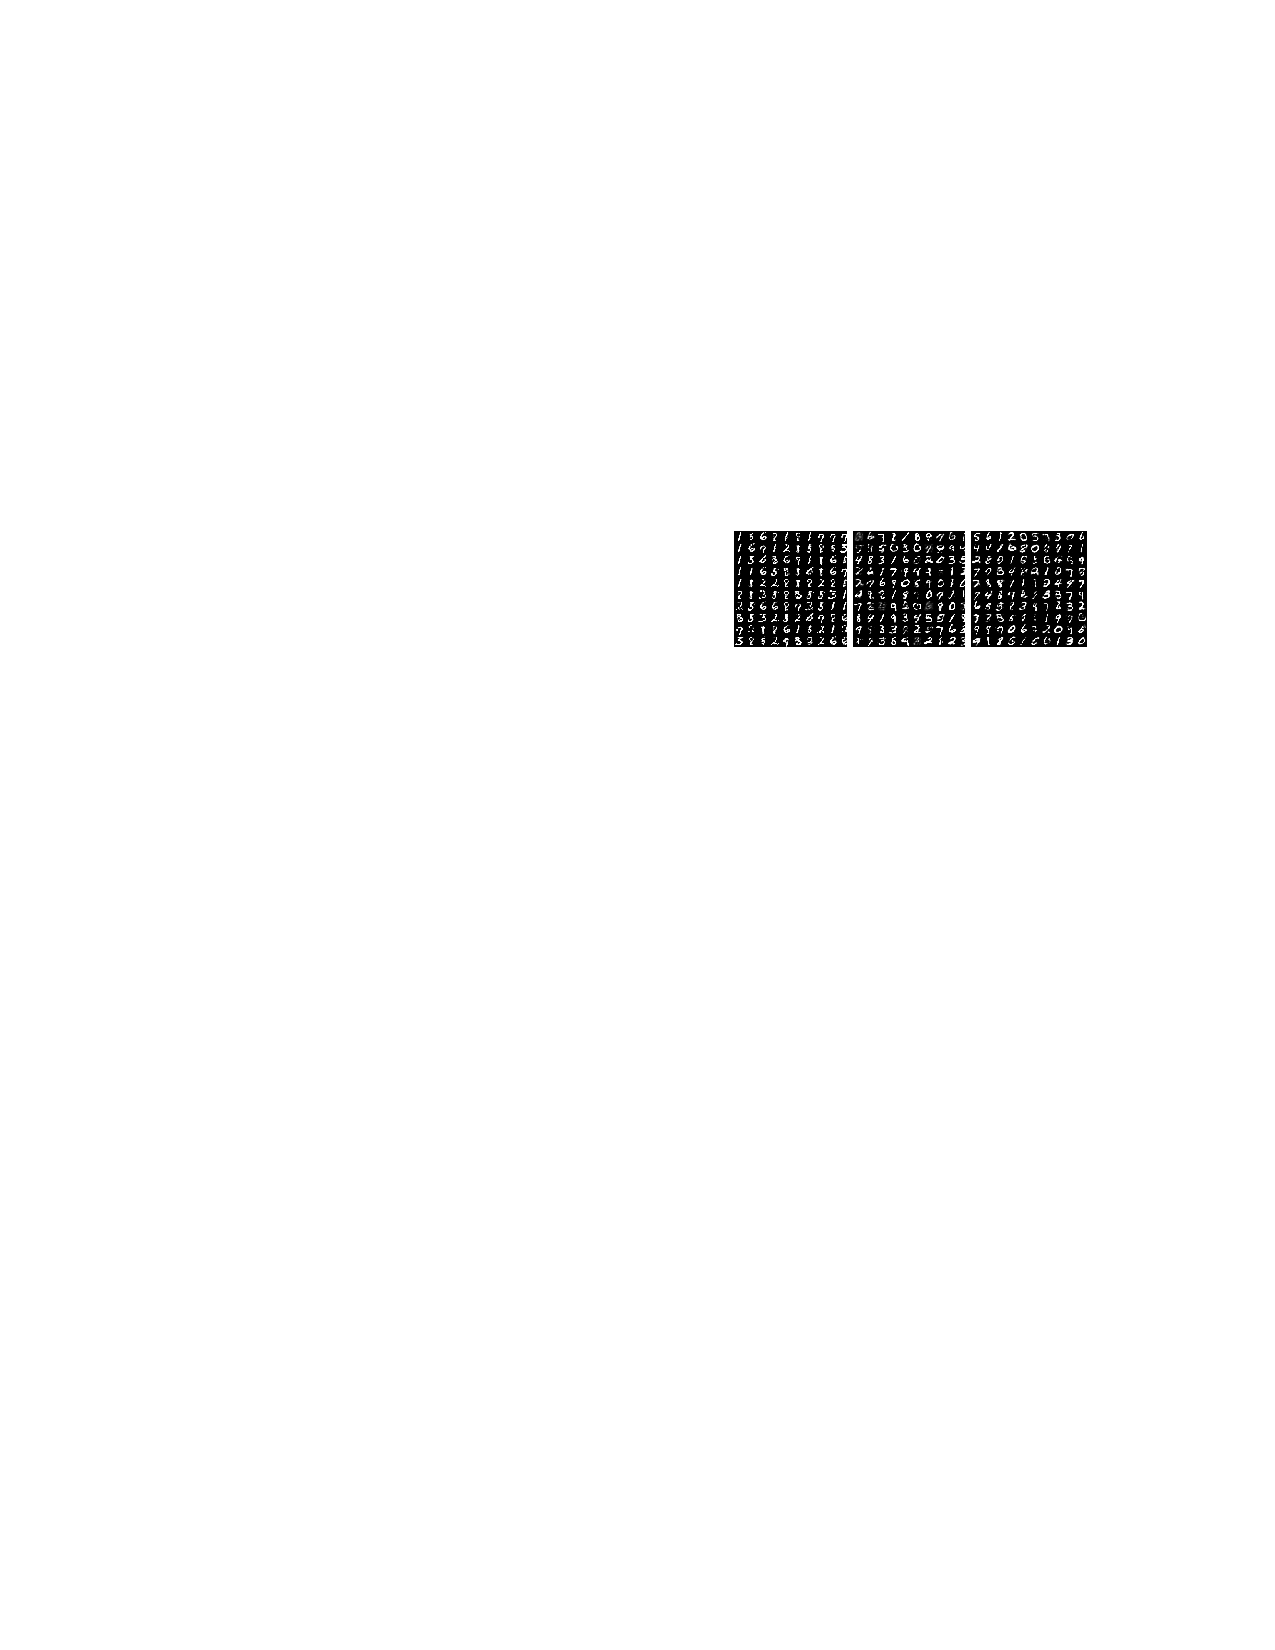
\includegraphics[width=0.5\columnwidth]{mnist_all.pdf}
% \caption{Performance of GAN (left), W-GAN (middle), SWG (right) on MNIST. (The figure is directly taken from \cite{deshpande2018generative}.) }
% \label{fig:mnistall}
% \end{figure}


\section{Additional Experimental Results}

\subsection{The Sliced Wasserstein Flow}
The whole code for the Sliced Wasserstein Flow was implemented in Python, for use with Pytorch\footnote{\url{http://www.pytorch.org}.}. The code was written so as to run efficiently on GPU, and is available on the publicly available repository related to this paper\footnote{\url{github.com/removed_for_double_blind}.}.

In practice, the SWF involves relatively simple operations, the most important being:
\begin{itemize}
  \item For each random $\theta\in\{\theta_n\}_{n=1\dots N_\theta}$,  compute its inner product with all items from a dataset and obtain the empirical quantiles for these \emph{projections}.
  \item At each step $k$ of the SWF, for each projection $z=\left<\theta, \bar{X}^i_k\right>$, apply two piece-wise linear functions, corresponding to the scalar optimal transport $\psi_{k, \theta}'(z)$.
\end{itemize}
Even if such steps are conceptually simple, the quantile and required linear interpolation functions were not available on GPU for any framework we could figure out at the time of writing this paper. Hence, we implemented them ourselves for use with Pytorch, and the interested reader will find them in the Github repository dedicated to this paper.

Given these operations, putting a SWF implementation together is straightforward, and the online code is able to apply it on any dataset.

\subsection{The need for dimension reduction through autoencoders}

In this study, we used an autoencoder trained on the dataset as a dimension reduction technique, so that the SWF is applied to transport particles in a latent space of dimension $d\approx 50$, instead of the original $d>1000$ of image data.

The curious reader may wonder why SWF is not applied directly to this original space, and what performances should be expected there. We have done this experiment, and we found out that SWF has much trouble rapidly converging to satisfying samples. In figure~\ref{fig:suppnoae}, we show the progressive evolution of particles undergoing SWF when the target is directly taken as the uncompressed dataset.

\begin{figure}
\centering
\includegraphics[width=\columnwidth]{figures/supplementary/fmnist_noae.pdf}
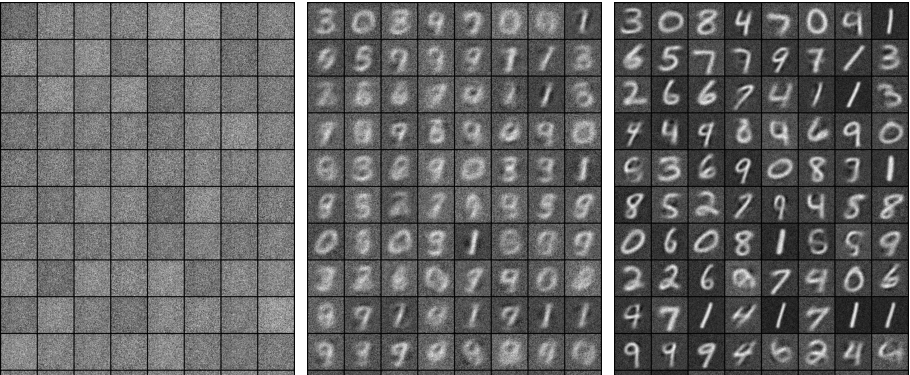
\includegraphics[width=\columnwidth]{figures/supplementary/mnist_noae.pdf}
\caption{The evolution of SWF through 15000 iterations, when the original high-dimensional data is kept instead of working on reduced bottleneck features as done in the main document. Showing results on the MNIST and FashionMNIST datasets.}
\label{fig:suppnoae}
\end{figure}

In this experiment, the strategy was to change the projections $\theta$ at each iteration, so that we ended up with a set of projections being $\{\theta_{n,k}\}_{n=1\dots N_\theta}^{k=1\dots K}$ instead of the fixed set of $N_\theta$ we now consider in the main document. This strategy is motivated by the complete failure we observed whenever we picked such fixed projections throughout iterations.

As may be seen on Figure~\ref{fig:suppnoae}, the particles definitely converge to samples from the desired datasets, and this is encouraging. However, we feel that the extreme number of iterations required to achieve such convergence comes from the fact that theory needs an integral over the $d-$dimensional sphere at each step of the SWF, which is clearly an issue whenever $d$ gets too large.
Although our solution of picking new samples from the sphere at each iteration alleviated this issue to some extent, the curse of dimensionality prevents us from doing much better with just thousands of \emph{random} projections at a time.

This being said, we are confident that good performance would be obtained if millions of random projections could be considered for transporting such high dimensional data because i/ theory suggests it and ii/ we observed excellent performance on reduced dimensions.

However, we, unfortunately, did not have the computing power it takes for such large scale experiments and this is what motivated us in the first place to introduce some dimension-reduction technique through AE.

\subsection{Structure of our autoencoders for reducing data dimension}

As mentioned in the text, we used autoencoders to reduce the dimensionality of the transport problem. The structure of these networks is the following:

\begin{itemize}
  \item $\textbf{Encoder}$ Four 2d convolution layers with \(num_chan_out, kernel size, stride, padding\) being $(3,3,1,1)$, $(32,2,2,0)$, $(32,3,1,1)$, $(32, 3,1,1)$, each one followed by a relu activation. At the output, a linear layer gets the desired bottleneck size.

  \item $\textbf{Decoder}$ A linear layer gets from the bottleneck features to a vector of dimension $8192$, which is reshaped as $(32, 16,16)$. Then, three convolution layers are applied, all with $32$ output channels and \(kernel size, stride, panning\) being respectively $(3,1,1)$, $(3,1,1)$, $(2,2,0)$. A 2d convolution layer is then applied with an output number of channels being that of the data \($1$ for black and white, $3$ for colour\), and a \(kernel size, stride, panning\) as $(3,1,1)$. In any case, all layers are followed by a relu activation, and a sigmoid activation is applied a the very output.
\end{itemize}

Once these networks defined, these autoencoders are trained in a very simple manner by minimizing the squared difference between input and output over the training set of the considered dataset (here MNIST or FashionMNIST). This training was achieved with the Adam algorithm \cite{kingma2014adam} with learning rate $1e-3$.

No additional training trick was involved as in Variational Autoencoder \cite{kingma2013VAE} to make sure the distribution of the bottleneck features matches some prior. The core advantage of the proposed method in this respect is indeed to turn any previously learned AE as a generative model, by automatically and non-parameterically transporting particles drawn from an arbitrary prior distribution $\mu$ to the observed empirical distribution $\nu$ of the bottleneck features over the training set.

\subsection{Convergence plots of SWF}

\begin{figure}
\begin{centering}
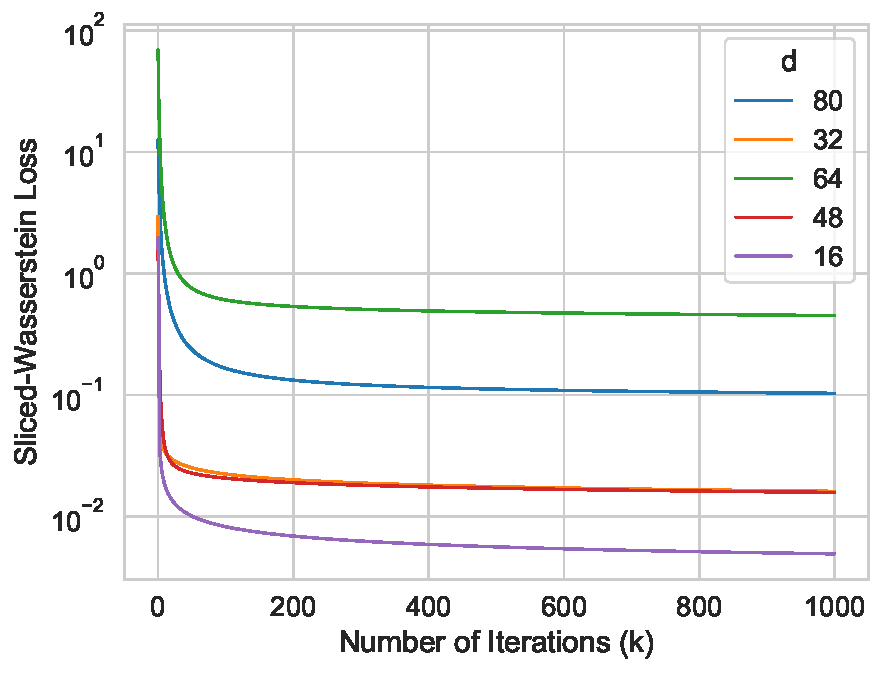
\includegraphics[width=0.5\columnwidth]{figures/iterations.pdf}
\par\end{centering}
\caption{Approximately computed $\SW$ between the output $\bar{\mu}_{k}^{N}$ and data distribution $\nu$ in the MNIST experiment for different dimensions $d$ for the bottleneck features (and the corresponding pre-trained AE).
\label{fig:supptoy_sw}}
\end{figure}

In the same experimental setting as in the main document, we also illustrate the behavior of the algorithm for varying dimensionality $d$ for the bottleneck-features. To monitor the convergence of SWF as predicted by theory, we display the approximately computed $\SW$ distance between the distribution of the particles and the data distribution. Even though minimizing this distance is not the real objective of our method, arguably, it is still a good proxy for understanding the convergence behavior.

Figure~\ref{fig:supptoy_sw} illustrates the results. We observe that, for all choices of $d$, we see a steady and smooth decrease in the cost for all runs, which is in line with our theory. The absolute value of the cost for varying dimensions remains hard to interpret at this stage of our investigations.

\section{Additional samples}

\subsection{Evolution throughout iterations}

In Figures~\ref{fig:suppmnist} and \ref{fig:suppfmnist} below, we provide the evolution of the SWF algorithm on the Fashion MNIST and the MNIST datasets in higher resolution, for an AE with $d=48$ bottleneck features.

\newcommand{\picwidth}{0.2}%originally 0.24
\begin{figure}
\centering
\includegraphics[width=\picwidth\columnwidth]{supplementary/mnist/train_image_0.png}
\includegraphics[width=\picwidth\columnwidth]{supplementary/mnist/train_image_10.png}
\includegraphics[width=\picwidth\columnwidth]{supplementary/mnist/train_image_20.png}
\includegraphics[width=\picwidth\columnwidth]{supplementary/mnist/train_image_30.png}\\
\includegraphics[width=\picwidth\columnwidth]{supplementary/mnist/train_image_40.png}
\includegraphics[width=\picwidth\columnwidth]{supplementary/mnist/train_image_50.png}

\includegraphics[width=\picwidth\columnwidth]{supplementary/mnist/train_image_100.png}
\includegraphics[width=\picwidth\columnwidth]{supplementary/mnist/train_image_200.png}
\caption{The evolution of SWF through 200 iterations on the MNIST dataset. Plots are for $1$, $11$, $21$, $31$, $41$, $51$, $101$ and $201$ iterations}
\label{fig:suppmnist}
\end{figure}

\begin{figure}
\centering
\includegraphics[width=\picwidth\columnwidth]{supplementary/alternative_fmnist/train_image_0.png}
\includegraphics[width=\picwidth\columnwidth]{supplementary/alternative_fmnist/train_image_10.png}
\includegraphics[width=\picwidth\columnwidth]{supplementary/alternative_fmnist/train_image_20.png}
\includegraphics[width=\picwidth\columnwidth]{supplementary/alternative_fmnist/train_image_30.png}\\
\includegraphics[width=\picwidth\columnwidth]{supplementary/alternative_fmnist/train_image_40.png}
\includegraphics[width=\picwidth\columnwidth]{supplementary/alternative_fmnist/train_image_50.png}

\includegraphics[width=\picwidth\columnwidth]{supplementary/alternative_fmnist/train_image_100.png}
\includegraphics[width=\picwidth\columnwidth]{supplementary/alternative_fmnist/train_image_200.png}
\caption{The evolution of SWF through 200 iterations on the FashionMNIST dataset. Plots are for $1$, $11$, $21$, $31$, $41$, $51$, $101$ and $201$ iterations}
\label{fig:suppfmnist}
\end{figure}

\subsection{Training samples, interpolation and extrapolation}

In Figures~\ref{fig:suppmnistsamples} and \ref{fig:suppfmnistsamples} below, we provide other examples of outcome from SWF, both for the MNIST and the FashionMNIST datasets, still with $d=48$ bottleneck features.

The most noticeable fact we may see on these figures is that while the actual particles which went through SWF, as well as linear combinations of them, all yield very satisfying results, this is however not the case for particles that are drawn randomly and then brought through a pre-learned SWF.

Once again, we interpret this fact through the curse of dimensionality: while we saw in our toy GMM example that using a pre-trained SWF was totally working for small dimensions, it is already not so for $d=48$ and only $3000$ training samples.

This noticed, we highlight that this generalization weakness of SWF for high dimensions is not really an issue, since it is always possible to i/ run SWF with more training samples if generalization is required ii/ re-run the algorithm for a set of new particles. Remember indeed that this does not require passing through the data again, since the distribution of the data projections needs to be done only once.
\renewcommand{\picwidth}{0.3}%originally 0.24


\begin{figure}
\centering
\subfigure[particles undergoing SWF]{
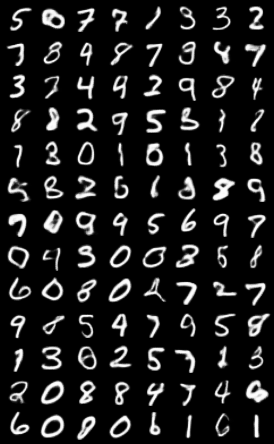
\includegraphics[width=\picwidth\columnwidth]{supplementary/MNIST_train_image_1000.png}}
\subfigure[After SWF is done: applying learned map on linear combinations of train particles]{
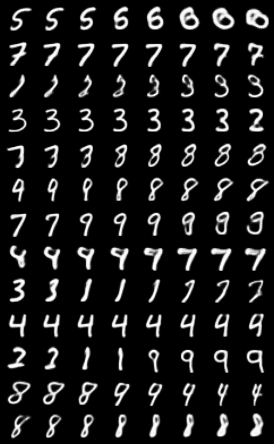
\includegraphics[width=\picwidth\columnwidth]{supplementary/MNIST_interp_image_1000.png}}
\subfigure[After SWF is done: applying learned map on random inputs.]{
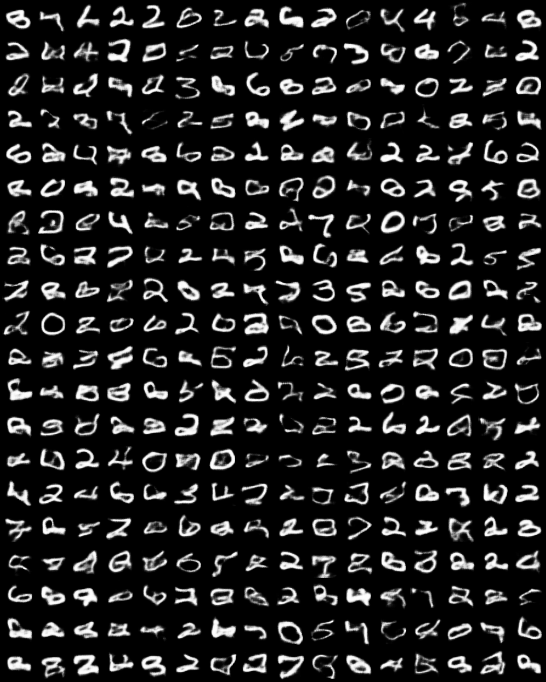
\includegraphics[width=\picwidth\columnwidth]{supplementary/MNIST_randomtest_image_1000.png}}
\caption{SWF on MNIST: training samples, interpolation in learned mapping, extrapolation.}
\label{fig:suppmnistsamples}
\end{figure}


\begin{figure}
\centering
\subfigure[particles undergoing SWF]{
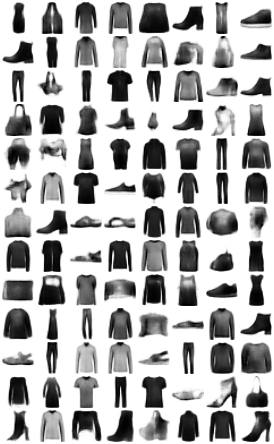
\includegraphics[width=\picwidth\columnwidth]{supplementary/FashionMNIST_train_image_1000.png}}
\subfigure[After SWF is done: applying learned map on linear combinations of train particles]{
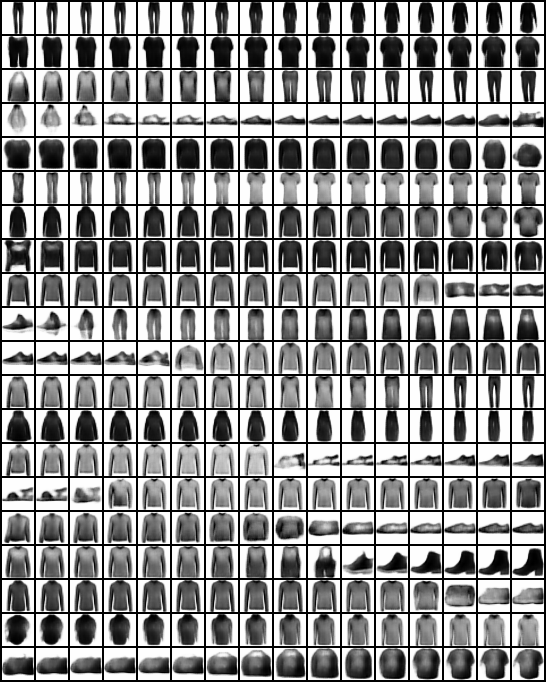
\includegraphics[width=\picwidth\columnwidth]{supplementary/FashionMNIST_interp_image_1000.png}}
\subfigure[After SWF is done: applying learned map on random inputs.]{
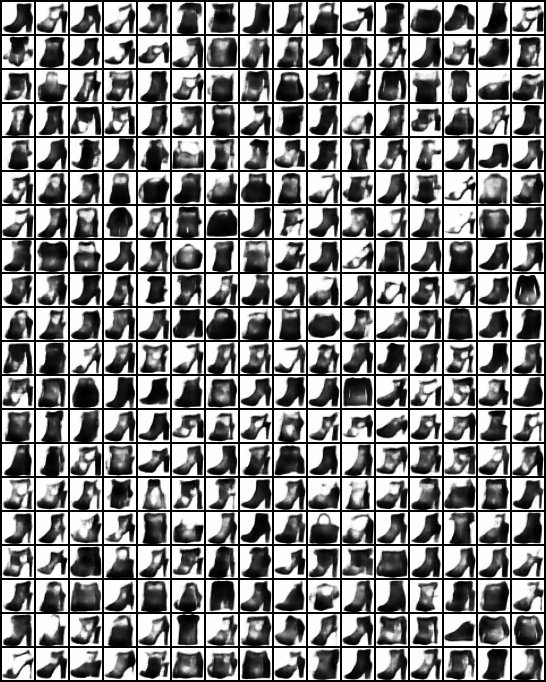
\includegraphics[width=\picwidth\columnwidth]{supplementary/FashionMNIST_randomtest_image_1000.png}}
\caption{SWF on FashionMNIST: training samples, interpolation in learned mapping, extrapolation.}
\label{fig:suppfmnistsamples}
\end{figure}







% \section{Details of Computing $(F_{\theta_{n}^*\#\hat{\mu}}^{-1} \circ F_{\theta^*_{n}\#\nu}) $}


% \umut{Antoine. -- sorting, interpolation etc}

% \begin{figure}
% \begin{centering}
% \setlength\tabcolsep{1pt}
% \begin{tabular}{cccccc}
% $\lambda=0$ & $\lambda=0.1$ & $\lambda=0.2$ & $\lambda=0.3$ & $\lambda=0.5$ & $\lambda=1$\tabularnewline
% 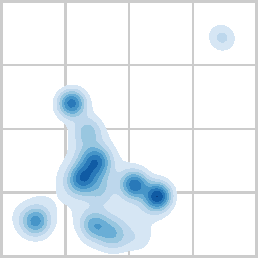
\includegraphics[width=2cm]{figures/supplementary/regularization/r0_output_dist_k=70-crop.pdf} & 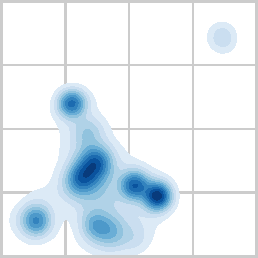
\includegraphics[width=2cm]{figures/supplementary/regularization/r01_output_dist_k=70-crop.pdf} & 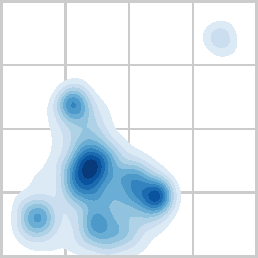
\includegraphics[width=2cm]{figures/supplementary/regularization/r02_output_dist_k=70-crop.pdf} &  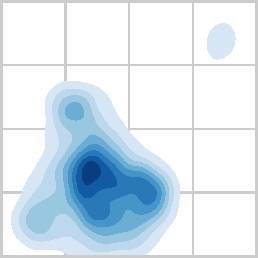
\includegraphics[width=2cm]{figures/supplementary/regularization/r03_output_dist_k=70-crop.pdf}&  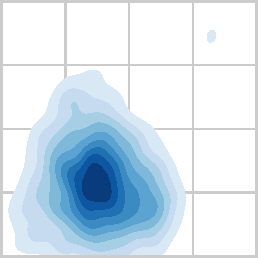
\includegraphics[width=2cm]{figures/supplementary/regularization/r05_output_dist_k=70-crop.pdf} &  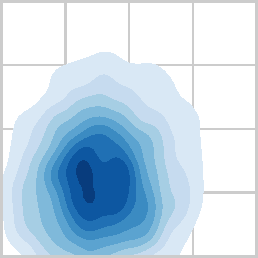
\includegraphics[width=2cm]{figures/supplementary/regularization/r1_output_dist_k=70-crop.pdf}
% \end{tabular}
% \par\end{centering}
% \caption{Influence of the regularization parameter $\lambda$. The higher $\lambda$, the more entropic the output distribution.\label{fig:lambda_supp}}
% \end{figure}


\bibliography{./references.bib}
\bibliographystyle{unsrt}

\end{document}
